\section{Oppgave 1 - GPIO}\label{sec:3-oppgave-GPIO}


\subsection{Beskrivelse}



I denne oppgaven skal vi skru på alle LED-ene i matrisen når knappen \verb|BUTTON 1| trykkes, og skru dem av når knappen \verb|BUTTON 2| trykkes. Dette gjøres med \verb|GPIO|-modulene. Dette er moduler som har ansvarer for generell input og output (\verb|GPIO| = \textbf{G}eneral \textbf{P}urpose \textbf{I}nput \textbf{O}utput).

Denne oppgaven er strukturert som en walkthrough for å introdusere konsepter som skal brukes i senere oppgaver. Tanken er at det blir gradvis mindre håndholding. Før dere starter er det lurt å skumlese appendiks \ref{app:datablad} og \ref{app:bit}. Utviklingsmiljøet kan også vise seg å være svært praktisk for å teste GPIO-modulen ved å sette registre live (se appendiks \ref{app:Debugging}).

I denne oppgaven, så trenger dere bare å endre på \verb|main.c|. De spesielt interesserte kan se på mappen \verb|.build_system| og \verb|Makefile|. Sistenevnte kan endres på om dere velger å lage flere \verb|.h| eller \verb|.c|-filer for at det skal bli ryddigere.

\begin{center}
 \begin{tabular}{|p{8.5cm} p{5.5cm}|} 
 \hline
 Filer & Skal denne filen endres?  \\ [0.5ex] 
 \hline\hline
 \verb|1_gpio/main.c| & \quad \quad \quad \quad ja  \\ 
 \hline
  \verb|1_gpio/.build_system| &  \quad \quad \quad \quad helst ikke \\ 
 \hline
 \verb|1_gpio/.vscode| &  \quad \quad \quad \quad helst ikke \\ 
 \hline
 \verb|1_gpio/Makefile| &  \quad \quad \quad \quad helst ikke \\ 
 \hline
\end{tabular}
\end{center}


\subsection{Oppgave}

LED-matrisen på nRF52 DK består av en 2x2 plassert rett over target MCU (se figur \ref{fig:interface-mcu}). Det er en GPIO-port assosiert med hver av LED-ene. Disser er aktivt lave, som vil si at vi må trekke porten lav dersom vi vil at LED-en skal lyse.

Til å starte oppgaven, ta en titt på den vedlagte filen \verb|PCA10040_Schematic_And_PCB.pdf| i mappen \verb|datablad|. Dette er referansedesignet for et nRF52832 DK. Finn først ut hvordan de to knappene \verb|BUTTON 1| og \verb|BUTTON 2| er koblet. 

\begin{itemize}
    \item Hvilke pinner på nRF52832-en brukes? Vil pinnene være høye eller lave dersom knappene trykkes?
\end{itemize}


Se deretter i databladet til nRF52832-serien (\texttt{nrf52832 Product Specification}). 

\begin{itemize}
    \item Hvordan ser minnekartet for mikrokontrolleren ut? Hva er baseadressen til \verb|GPIO|-modulene? Bytt ut \verb|__GPIO_BASE_ADDRESS0__| i \verb|main.c| med den faktiske baseadressen. 
\end{itemize}

I \verb|main.c| vil dere se at det er definert et \verb|struct| som heter \verb|NRF_GPIO_REGS0|. Dette \verb|struct|-et representerer alle registrene til \verb|GPIO|-modulen. Ved å typecaste adressene til \verb|GPIO|-modulen inn i \verb|struct|-en, kan vi så endre på \verb|struct|-en medlemsvariabler for så å skrive direkte til registrene (Typisk \textit{memory mapped IO} \verb|struct|). Det er nettopp dette som er formålet med kodelinjen:

\verb|#define GPIO0 ((NRF_GPIO_REGS0*)__GPIO_BASE_ADDRESS0__)|

Når denne er definert, kan vi eksempelvis endre \verb|OUT|-registret ved å kalle:

\verb|GPIO0->OUT = desired_value;|\newline

 Dere vil også se at medlemsvariabelen \verb|RESERVED0| i \verb|GPIO0| er en array av type \verb|volatile| \verb|uint32_t| med 321 elementer. Dette er fordi databladet forteller oss at \verb|OUT|-registeret i modulen \verb|GPIO0| har et offsett på 
 \verb|0x504| ($\text{504}_{\text{16}}$) fra modulens baseadresse. $\text{504}_{\text{16}}$ er det samme som $\text{1284}_{\text{10}}$. Altså er det 1284 byte mellom baseadressen og \verb|OUT|-registeret. Siden vi bruker en ordstørrelse (word) på 32 bit, deler vi dette tallet på fire (32 bit er 4 byte). Altså, 1284/4 = 321. I hexadesimal, tilsvarer dette \verb|0x141|.
 
 \begin{itemize}
     \item Dersom man nå følger samme resonnement, hva skal \verb|__RESERVED1_SIZE__| være? Finn ut dette, og endre \verb|main.c| tilsvarende.
 \end{itemize}


Når dere har gjort det, kan dere fylle ut de manglende bitene i \verb|main()|, som består av å legge inn logikk slik at LED-matrisen lyser når vi trykker på knapp \verb|BUTTON 1|, og skrur seg av når vi trykker på knapp \verb|BUTTON 2|. Dersom dere nå kaller \verb|make| og \verb|make flash| i terminalen, vil dere kunne se at LED-matrisen lyse av og på, avhengig av hvilken knapp som blir trykket, om alt har blitt gjort riktig.


\subsection{Hint}\label{subsec:GPIO-hint}

\begin{itemize}
    \item Det er fort gjort å forveksle \verb|GPIO| med \verb|GPIOTE|-modulen (\verb|GPIO| \textbf{T}asks
and \textbf{E}vents). Sistnevnte brukes for å lage et hendelsesbasert system, og brukes ikke i denne oppgaven.
    \item Om dere skriver inn \verb|GPIO|-modulenes baseadresse i base 16 (heksadesimal), må dere huske \verb|0x| foran adressen. Hvis ikke vil kompilatoren
    tro dere mener base 10.
    \item Når dere skal finne \verb|__RESERVED1_SIZE__|, så husk at \verb|DETECTMODE| starter på \verb|0x524|, som betyr at den byten slutter på \verb|0x527|. Altså starter ikke \verb|RESERVED1| på \verb|0x524|, men på \verb|0x528|.
    \item \verb|BTN| brukes veldig ofte som en forkortelse for \textit{button}.
    \item Sjekk ut appendiks \ref{app:bit} for hvordan man kan manipulere bits.
    \item Sjekk ut appendiks \ref{app:datablad} for hvordan man bruker databladet til å typecaste.

\end{itemize}


\section{Oppgave 2 - UART}\label{sec:4-oppgave-UART}

\subsection{Beskrivelse}

I denne oppgaven skal vi sette opp toveis kommunikasjon mellom datamaskinen og nRF52 DK. Dette gjøres med \verb|UART| (\textbf{U}niversal \textbf{A}synchronous \textbf{R}eceiver-\textbf{T}ransmitter, se gjerne videoforelesninger om dette). Tradisjonelt ble signalene mellom to \verb|UART|-moduler ofte overført via et RS232-COM grensesnitt. På Sanntidssalen finnes det en DSUB9-port som vi kunne brukt til dette, men i denne øvingen trenger vi ikke det. 

Som nevnt i introduksjonen kommuniserer vi med target MCU gjennom en interface MCU. Dette er en nRF5340 mikrokontroller som lar oss programmere nRF52832-SoCen over USB. I tillegg til dette implementerer den en USB CDC (\textbf{C}ommunications \textbf{D}evice \textbf{C}lass), som lar oss \textit{pakke inn} \verb|UART|-signaler i USB-pakker. På den måten vil datamaskinen se ut som en \verb|UART|-enhet for mikrokontrolleren, og mikrokontrolleren vil i gjengjeld se ut som en USB-enhet for datamaskinen.

Les kjapt appendiks \ref{app:uart} før dere begynner. Appendikset vil gi dere en kort introduksjon til \verb|UART|, og litt spesifikk informasjon om begrensningene som kan oppstå ved bruk av \verb|UART| i nRF52 DK.

I denne oppgaven, så trenger dere ikke å endre noe som helst annet enn \verb|Makefile|. Dette er fordi dere skal implementere en \verb|main.c| selv som bruker logikk fra \verb|GPIO|-modulene til å kommunisere med en datamaskin via \verb|UART|-modulen som dere kommer til å lage.

\begin{center}
 \begin{tabular}{|p{8.5cm} p{5.5cm}|} 
 \hline
 Filer & Skal denne filen endres?  \\ [0.5ex] 
 \hline\hline
  \verb|2_uart/gpio.h| & \quad \quad \quad \quad nei  \\ 
  \hline
  \verb|2_uart/.build_system| &  \quad \quad \quad \quad helst ikke \\ 
  \hline
    \verb|2_uart/.vscode| &  \quad \quad \quad \quad helst ikke \\ 
 \hline
 \verb|2_uart/Makefile| &  \quad \quad \quad \quad ja \\ 
 \hline
\end{tabular}
\end{center}


\subsection{Oppgave - Innføring i UART}

Det første vi må gjøre er å identifisere hvor \verb|UART|-pinnene faktisk er koblet. For å finne dette ut, tar dere en titt i \verb|PCA10040_Schematic_And_PCB.pdf|. 

\begin{itemize}
    \item Finn ut hvilken pinne fra nRF52832-brikken som er merket \verb|UART_INT_RX|, og hvilken pinne som er \verb|UART_INT_TX|.
\end{itemize}

 Disse pinnene skal vi senere konfigurere som henholdsvis input og output.
 
 \begin{itemize}
     \item Opprett deretter filene \verb|uart.h| og \verb|uart.c|. Headerfilen skal inneholde deklarasjonen til tre funksjoner:

\begin{lstlisting}
void uart_init();
void uart_send(char letter);
char uart_read();
\end{lstlisting} 
Disse funksjonene skal brukes for å manipulere \verb|UART|-modulen i mikrokontrolleren. De må derfor inkluderes fra \verb|main.c|.
 \end{itemize}
 
 I implementasjonsfilen (\verb|uart.c|) skal vi igjen bruke memory mapped IO, slik vi gjorde for \verb|GPIO0| med \verb|struct|-er til minneoperasjoner:
 
 \begin{itemize}
    \item Opprett en \verb|struct| som dere skal typecaste til \verb|UART|-modulen. Gi denne navnet \verb|NRF_UART_REG|.
\end{itemize}

Som dere kanskje har merket, så har det ikke blitt inkludert en \verb|main.c| i mappen for denne oppgaven. Det er opp til dere å opprette denne. Om man sitter litt fast på akkuratt dette, kan det være hensiktsmessig å ta inspirasjon fra \verb|main.c| fra oppgave \ref{sec:3-oppgave-GPIO}.





\cprotect\subsubsection{\lstinline{void uart_init()}}
Målet med denne funksjonen er å initialisere de nødvendige \verb|GPIO|-pinnene som input/output. 


\begin{itemize}
    \item Første steg er derfor å inkludere \verb|gpio.h| (allerede implementert for dere) i \verb|uart.c|
    \item Andre steg er å konfiguere pinnene som input eller output i \verb|GPIO|-modulen.
    \item Når pinnene er ferdig konfigurert i \verb|GPIO|-modulene, må de brukes av \verb|UART|-modulen. Dette gjøres med \verb|PSELTXD|- og \verb|PSELRXD|-registrene.
\end{itemize}



Om dere ser i \verb|PCA10040_Schematic_And_PCB.pdf|, vil dere se at vi ikke har noen \verb|CTS|- eller \verb|RTS|-koblinger fra nRF52-brikken til interface-brikken. 

\begin{itemize}
    \item Dere må derfor velge en baudrate på 9600 for å unngå pakketap på grunn av mangel på flytkontroll i hardware (sjekk ut registeret \verb|BAUDRATE|).
    \item I tillegg er det viktig å faktisk fortelle \verb|UART|-modulen at vi ikke har \verb|CTS|- eller \verb|RTS|-koblinger. Sett opp de riktige registrene for dette (sjekk ut \verb|PSELRTS| og \verb|PSELCTS|).
    \item 

Til slutt skal vi gjøre to ting. Først må vi skru på \verb|UART|-modulen, som gjøres med et eget \verb|ENABLE|-register. Deretter skal vi starte å ta imot meldinger, sjekk derfor ut \verb|TASKS_STARTRX|-registeret. 
\end{itemize}







\cprotect\subsubsection{\lstinline{void uart_send(char letter)}}

Denne funksjonen skal ta i mot en enkel bokstav, for å sende den over til datamaskinen.

Sjekk ut figur 163 (\textit{UART Transmission} i side 536) i databladet til nRF52-serien for å finne ut hva dere skal gjøre. Husk å vente til sendingen er ferdig, før dere skrur av sendefunksjonaliteten.


\cprotect\subsubsection{\lstinline{char uart_read()}}

Denne funksjonen skal lese en bokstav fra datamaskinen og returnere den. Vi ønsker ikke at funksjonen skal blokkere, så om det ikke er en bokstav klar akkurat når den kalles, skal den returnere \verb|'\0'|.

Husk at dere må ta hensyn til rekkefølge for å kunne garantere at \verb|UART|-modulen ikke taper informasjon.

\begin{itemize}
    \item I praksis kan pakketap unngå ved å sette \verb|EVENTS_RXDRDY| til \verb|0| før \verb|RXD| blir lest.
    \item I tillegg er det viktig å sørge for å kun lese \verb|RXD| en gang. Altså: dere skal ikke skru av mottakerregisteret når dere har lest meldingen.
\end{itemize}
\subsection{Sendefunksjon}
Programmer deretter micro:bit-en til å sende \verb|A| om knappen \verb|BUTTON 1| trykkes, og \verb|B| om \verb|BUTTON 2| trykkes i \verb|main.c|.

For å motta meldingene på datamaskinen, bruker vi på Sanntidslabben programmet \verb|picocom|. Kall dette fra et terminalvindu:

\verb|picocom -b 9600 /dev/ttyACM0|

for å fortelle \verb|picocom| at det skal høre etter enheten \verb|/dev/ttyACM0|, med en baudrate på 9600 bit per sekund.

For å avslutte \verb|picocom| er det \verb|Ctrl+A| etterfulgt av \verb|Ctrl+X|.

\subsection{Mottaksfunksjon}
Deretter, lytt etter sendte pakker på utviklingskitet. Om datamaskinen har sendt en bokstav, skal mikrokontrolleren skru på LED-matrisen om den var av, og skru den av om den allerede var på. Denne logikken implementerer dere i \verb|main.c|

For å sende bokstaver fra datamaskinen bruker vi igjen \verb|picocom|. Standardoppførselen til \verb|picocom| er å sende alle bokstaver som skrives inn i terminalen når det kjører. Bokstavene vil derimot ikke bli skrevet til skjermen, så dere vil ikke få noen visuell tilbakemelding på datamaskinen (gitt at dere ikke manuelt sender bokstaven tilbake). Sjekk ut appendiks \ref{app:picocom} dersom dere vil ha mer informasjon om \verb|picocom|, eller om dere får feilmeldinger.


\subsection{Oppgave - Mer avansert IO}

Nå har dere en funksjon for å sende over nøyaktig en bokstav av gangen; og en funksjon for å motta nøyaktig en bokstav av gangen. Om vi ønsker å sende en en \verb|C|-streng av vilkårlig lengde må vi lage en funksjon som dette:

\begin{lstlisting}
void uart_send_str(char ** str){
        UART->TASKS_STARTTX = 1;
        char * letter_ptr = *str;
        while(*letter_ptr != \0){
                UART->TXD = *letter_ptr;
                while(!UART->EVENTS_TXDRDY);
                UART->EVENTS_TXDRDY = 0;
                letter_ptr++;
        }
}
\end{lstlisting}


Dette er egentlig en dårlig implementasjon, ettersom den gjør nesten det samme som \verb|printf|, uten noen av formateringsalternativene som gjør \verb|printf| ettertraktet. Det er derfor litt lurere å inkludere \verb|<stdio.h>| og bruke en heltallsvariant av \verb|printf|, kalt \verb|iprintf|. Det er derimot litt problematisk å bruke \verb|iprintf| direkte, ettersom den i utgangspunktet snakker med \verb|stdout|, som tradisjonelt sett peker til en terminal. Derfor bruker vi heller et bibliotek kalt \verb|newlib| som er en variant av \verb|<stdio.h>| for tilpassede datamaskiner.

Når \verb|printf(...)| kalles, vil et annet funksjonskall til \verb|_write_r(...)| utføres i bakgrunnen. Denne funksjonen vil deretter kalle \lstinline{ssize\_t \_write(int fd, const void * buf, size\_t count)}, som foreløpig ikke gjør noe. Grunnen til at denne finnes, er at den trengs for at programmet skal kompilere, men den er i utgangspunktet tom, fordi vi gir lenkeren flagget \verb|--specs=nosys.specs| (sjekk \verb|Makefilen|).

Med \verb|newlib| kan vi lage mange varianter av slike skrivefunksjoner om vi har et komplekst system med mange skriveenheter eller om vi har flere tråder. Denne arkitekturen har bare en kjerne og vi vil bare bruke \verb|UART|, så vi kan fint implementere en global variant av denne skrive funksjonen. For å gjøre det, legger vi til følgene i \verb|main.c|:


\begin{lstlisting}
#include <stdio.h>

[...]

ssize_t _write(int fd, const void *buf, size_t count){
        char * letter = (char *)(buf);
        for(int i = 0; i < count; i++){
                uart_send(*letter);
                letter++;
        }
        return count;
}
\end{lstlisting}

Merk at returtypen til \lstinline{\_write} er \lstinline{ssize\_t}, mens \verb|count|-variabelen er av type \verb|size_t|. Når denne funksjonen er implementert, kan dere kalle eksempelvis skrive:




\verb|iprintf("The average grade in TTK%d was in %d was: %c\n\r",4235|\newline
\verb|,2022,'B')|

Om \verb|picocom| da forteller dere gjennomsnittskarakteren i tilpassede datasystemer i 2022, så har dere fullført oppgaven.




\cprotect\subsection{Oppgave - \lstinline{_read()} (Frivillig)}

Vi kan også implementere funksjonen \lstinline{ssize_t_read(int fd, void *buf, size_t count)}, slik at vi kan bruke \verb|scanf| fra \verb|<stdio.h>|. Legg til denne funksjonen i main-filen:


\begin{lstlisting}
ssize_t _read(int fd, void *buf, size_t count){
        char *str = (char *)(buf);
        char letter;
        
        do {
                letter = uart_read();
        } while(letter == 
        \0
        );
        
        *str = letter;
        return 1;
}
\end{lstlisting}

Skriv deretter et kort program som spør datamaskinen etter 2 heltall. Disse
skal leses inn til micro:bit-en, som vil gange dem sammen, og sende resultatet
tilbake til datamaskinen.

\subsection{Hint}\label{subsec:UART-hint}

\begin{itemize}
    \item På nRFen er det nyttig å tenke på \verb|UART|-modulen som en tilstandsmaskin, der den vil sende så lenge den er i tilstanden \verb|TASKS_STARTTX|. Den vil bare stoppe å sende når den forlater denne tilstanden, altså når den går over i \verb|TASKSSTOPX| (sjekk side 537 i referansemanualen).
    \item Det skal være totalt 12 reserverte minneområder i \verb|UART|-\verb|struct|-en. De skal ha følgende størrelser: 3, 56, 4, 1, 7, 46, 64, 93, 31, 1, 1, 17.
    \item Det er er ingen fysisk forskjell på tasks, events og vanlige registre annet enn hva de brukes til. Når \verb|LSB| er satt i et event-register, har en hendelse skjedd, mens når \verb|LSB| settes i et task-register, startes en oppgave.
    \item \lstinline{int fd i _read og _write} står for \textit{file descriptor}. Den er der i tilfelle noen vil bruke \verb|newlib| i forbindelse med et operativsystem. I denne oppgaven lar vi denne være som den er.
    \item Husk å legge til \verb|uart.c| i Makefilen, bak \verb|SOURCES := main.c|.
\end{itemize}






\section{Oppgave 3: GPIOTE og PPI}
\subsection{Beskrivelse}


Akkurat nå jobber vi med en mikrokontroller som er basert på en ARM Cortex M4 prosessor som bare har en kjerne. Vi har derfor ikke mulighet til å kjøre kode i sann parallellisering. En mulighet er å bytte veldig fort mellom to eller flere oppgaver (også kalt fibre) samtidig, men dette kan være problematisk om man trenger nøyaktige tidsfrister for programmene vi skriver.

For å løse dette problemenet, har nRF52832-en noe som kalles \verb|PPI| (\textbf{P}rogrammable \textbf{P}eripheral \textbf{I}nterconnect). Dette er en teknologi som lar oss direkte koble en periferienhet til en annen, uten at vi trenger å kommunisere først med CPU-en. For å dra nytte av denne teknologien, må vi innføre oppgaver og hendelser (tasks og events). Disse er egentlig bare registre, men brukes litt annerledes enn vanlig registre. Om et hendelsesregister inneholder verdien \verb|1| - så har en hendelse inntruffet. Om den derimot inneholder \verb|0|, så har ikke hendelsen inntruffet. Oppgaveregistrene er knyttet til gitte oppgaver, som startes ved å skrive verdien \verb|1| til det. Det som er litt spesielt, er at oppgaven ikke kan stanses ved å skrive verdien \verb|0| til samme register som startet oppgaven.

De fleste periferienhetene som finnes på nRF52832-en har noen form for oppgaver og hendelser. For å knytte disse til \verb|GPIO|-pinnene, har vi en egen modul kalt \verb|GPIOTE| (\textbf{G}eneral \textbf{P}urpose \textbf{I}nput \textbf{O}utput \textbf{T}asks and \textbf{E}vents). I denne oppgaven skal vi bruke \verb|GPIOTE|-modulen til å definere en hendelse (\verb|BUTTON 1| trykket), og fire oppgaver (skru på eller av LED-matrisen).


I denne oppgaven, så får dere igjen utlevert ferdig \verb|gpio.h|. I tillegg, så får dere halvferdige \verb|.h|-filer for \verb|PPI| og \verb|GPIOTE|-modulene som dere selv skal implementere. Som i forrige oppgave, skal dere selv implementere de tilhørende \verb|.c|-filene og en \verb|main.c|-fil. Dere må derfor også endre \verb|Makefile|.

\begin{center}
 \begin{tabular}{|p{8.5cm} p{5.5cm}|} 
 \hline
 Filer & Skal denne filen endres?  \\ [0.5ex] 
 \hline\hline
 \verb|3_gpiote/gpio.h| & \quad \quad \quad \quad nei  \\ 
 \hline
  \verb|3_gpiote/ppi.h| & \quad \quad \quad \quad ja  \\ 
  \hline
  \verb|3_gpiote/gpiote.h| & \quad \quad \quad \quad ja  \\ 
  \hline
  \verb|3_gpiote/.build_system| &  \quad \quad \quad \quad helst ikke \\ 
 \hline
 \verb|3_gpiote/.vscode| &  \quad \quad \quad \quad helst ikke \\ 
 \hline
 \verb|3_gpiote/Makefile| &  \quad \quad \quad \quad ja \\ 
 \hline
\end{tabular}
\end{center}



\subsection{Oppgave - Grunnleggende GPIOTE og PPI}
Først LED-matrisen konfigureres og lysene skrus av. Dere trenger ikke å konfigurere forsyningspinnene fordi \verb|GPIOTE|-modulen vil ta hånd om dette for dere. På samme måte slipper dere å konfigurere \verb|BUTTON 1| som input.

Dere har allerede fått utlevert headerfilene \verb|gpiote.h| og \verb|ppi.h| uten riktig informasjon. Dere må selv lese kapitlene om \verb|GPIOTE| og \verb|PPI| for å se hvordan de skal brukes og hva som skal fylles inn før dere kan bruke dem. Når dette er gjort, skal dere gjøre følgende:

\subsubsection{GPIOTE}

Fem \verb|GPIOTE|-kanaler skal brukes. 

\begin{itemize}
    \item Bruk en kanal til å lytte til \verb|BUTTON 1|. Denne kanalen skal genere en hendelse når knappen trykkes. 
    \item De resterende kanalene skal alle være konfigurert som oppgaver, og koblet til hver sin forsyningspinne for LED-matrisen. Forsyningsspenningen skal veksle hver gang oppgaven aktiveres. Hvilken initialverdi disse \verb|GPIOTE|-kanalene har er opp til dere.
\end{itemize}

\subsubsection{PPI}

For å koble \verb|BUTTON 1|-knapphendelsen til forsyningsoppgavene, trenger vi fire \verb|PPI|-kanaler; en for hver forsyningspinne. Som dere ser i databladet, kan hver \verb|PPI|-kanal konfigureres med en peker til en hendelse, og en peker til en oppgave. Fordi vi lagrer pekerene i registre på hardware, må vi typecaste hver peker til en \texttt{uint32\_t}, som demonstrert her:

\verb|PPI->PPI_CH[0].EEP = (uint32_t)&(GPIOTE->EVENTS_IN[4]);|\newline
\verb|PPI->PPI_CH[0].TEP = (uint32_t)&(GPIOTE->TASKS_OUT[0]);|


Denne kodesnutten setter registeret \verb|EventEndPoint| for \verb|PPI|-kanal \verb|0| til adressen av \verb|GPIOTE-EVENTS_IN[4]| - typecastet til en \verb|uint32_t|. Tilsvarende vil den sette registeret \verb|TaskEndPoint| for \verb|PPI|-kanal \verb|0| til adressen av \verb|GPIOTE->TASKS_OUT[0]| etter å ha typecastet den til en \verb|uint32_t|.


Denne koden kan være litt kryptisk første gang man ser den, men om man tar seg litt tid til å lage en mental modell av hvor hver peker går, så ser man ganske fort at det er egentlig veldig rett frem. 

\begin{itemize}
    \item Sett de ulike \verb|PPI|-registrene til riktige verdier.
\end{itemize}


\subsubsection{Opphold CPU}

Når den ene \verb|GPIOTE|-hendelsen er koblet til de fem \verb|GPIOTE|-oppgavene gjennom \verb|PPI|-kanalene, skal LED-matrisen veksle mellom å være av eller på hver gang \verb|BUTTON 1| trykkes - uavhengig av hva CPU-en gjør. Test dette ut ved å lage en evig løkke hvor CPU-en ikke gjør noe nyttig arbeid (altså tom).

Når dere har kompilert og flashet programmet over til utviklingskitet, skal LED-matrisen fungere som beskrevet. Det kan allikevel hende at matrisen ved enkelte knappetrykk blinker fort av og på, eller ikke veksler i det hele. Grunnen til dette er et fenomen kalt \textit{input bounce}.

Ideelt sett, ville spenningen til \verb|BUTTON 1| sett ut som en spenningskurven til en ideell bryter (se figur \ref{fig:bryter}). I virkeligheten vil de mekaniske platene i bryteren gjentatt slå mot-, og sprette fra hverandre. Når dette skjer, får vi spenningskurven for den reelle bryteren i figur \ref{fig:bryter} I dette tilfellet kan CPU-en registrere spenningstransienten som raske knappetrykk.

\begin{figure}[ht]
    \centering
    

\tikzset{every picture/.style={line width=0.75pt}} %set default line width to 0.75pt        

\resizebox{.85\textwidth}{!}{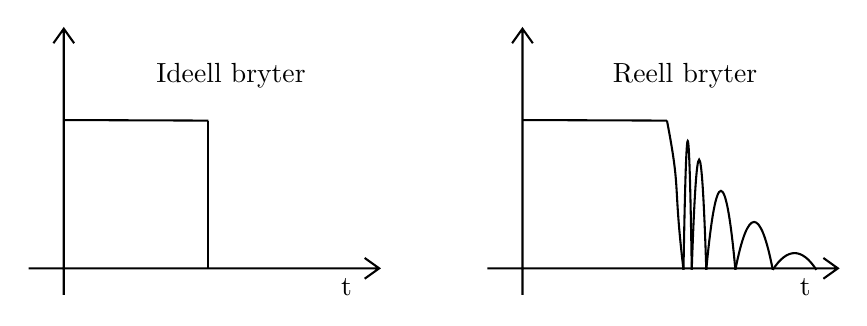
\begin{tikzpicture}[x=0.75pt,y=0.75pt,yscale=-1,xscale=1]
%uncomment if require: \path (0,300); %set diagram left start at 0, and has height of 300

%Shape: Axis 2D [id:dp9901238578898577] 
\draw  (33,170.45) -- (201.86,170.45)(49.89,55) -- (49.89,183.27) (194.86,165.45) -- (201.86,170.45) -- (194.86,175.45) (44.89,62) -- (49.89,55) -- (54.89,62)  ;
%Shape: Axis 2D [id:dp6811118948253481] 
\draw  (254,170.45) -- (422.86,170.45)(270.89,55) -- (270.89,183.27) (415.86,165.45) -- (422.86,170.45) -- (415.86,175.45) (265.89,62) -- (270.89,55) -- (275.89,62)  ;
%Straight Lines [id:da4843943952741787] 
\draw    (50,99) -- (119.5,99.27) ;
%Straight Lines [id:da293121433985875] 
\draw    (119.5,99.27) -- (119.5,170.27) ;
%Straight Lines [id:da6762241711099313] 
\draw    (271,99) -- (340.5,99.27) ;
%Shape: Parabola [id:dp5439190691797124] 
\draw   (352.45,171.11) .. controls (351.19,88.44) and (349.86,88.44) .. (348.47,171.11) ;
%Shape: Parabola [id:dp8649858969152793] 
\draw   (359.45,171.12) .. controls (357.18,100.44) and (354.84,100.44) .. (352.45,171.11) ;
%Shape: Parabola [id:dp36725763713463566] 
\draw   (373.47,171.13) .. controls (368.84,120.43) and (364.17,120.43) .. (359.45,171.12) ;
%Shape: Parabola [id:dp4674702723898885] 
\draw   (391.48,171.15) .. controls (385.5,140.42) and (379.49,140.42) .. (373.47,171.13) ;
%Shape: Parabola [id:dp8011958280177405] 
\draw   (412.49,171.16) .. controls (405.5,160.42) and (398.5,160.41) .. (391.48,171.15) ;
%Curve Lines [id:da6229326940059043] 
\draw    (340.5,99.27) .. controls (347.33,134.63) and (343.33,127.63) .. (348.47,171.11) ;

% Text Node
\draw (182,174) node [anchor=north west][inner sep=0.75pt]   [align=left] {t};
% Text Node
\draw (403,174) node [anchor=north west][inner sep=0.75pt]   [align=left] {t};
% Text Node
\draw (253,67) node [anchor=north west][inner sep=0.75pt]   [align=left] {\si{\V}};
% Text Node
\draw (33,67) node [anchor=north west][inner sep=0.75pt]   [align=left] {\si{\V}};
% Text Node
\draw (93,70) node [anchor=north west][inner sep=0.75pt]   [align=left] {Ideell bryter};
% Text Node
\draw (313,70) node [anchor=north west][inner sep=0.75pt]   [align=left] {Reell bryter};


\end{tikzpicture}}
    \caption{Spenningen over en ideell- og en reell bryter.}
    \label{fig:bryter}
\end{figure}

Stort sett er det tre grunner til at dette ikke er et problem:

\begin{enumerate}
    \item Vi har tactile pushbuttons på utviklingskitet. Disse er mye bedre på å redusere bounce enn andre typer knapper.
    \item Utvilkingskitet har debouncer-kretser for hver bryter, som reduserer problemet.
    \item I tillegg, dersom man manuelt sjekker knappeverdien i software, vil CPU-en som oftest ikke være rask nok til å merke at transienten er der. Dette er grunnen til at dere sannsynligvis ikke hadde dette problemet da dere brukte \verb|GPIO|-modulen.
\end{enumerate}

\subsection{Hint}\label{subsec:PPI-hint}


\begin{itemize}
    \item Husk å aktivere hver \verb|PPI|-kanal. Når de er konfigurert riktig, aktiveres de ved å skrive til \verb|CHENSET| i \verb|PPI|-instansen (husk at vi bare bruker seks \verb|PPI|-kanaler totalt).
    \item \verb|GPIOTE|-kanalene trenger ingen eksplisitt aktivering fordi \verb|MODE|-feltet i \verb|CONFIG|-registeret automatisk tar hånd om pinnen for dere.
\end{itemize}
